%!TEX root = ../template.tex
%%%%%%%%%%%%%%%%%%%%%%%%%%%%%%%%%%%%%%%%%%%%%%%%%%%%%%%%%%%%%%%%%%%%
%% chapter4.tex
%% NOVA thesis document file
%%
%% Chapter with lots of dummy text
%%%%%%%%%%%%%%%%%%%%%%%%%%%%%%%%%%%%%%%%%%%%%%%%%%%%%%%%%%%%%%%%%%%%

\typeout{NT FILE chapter4.tex}%

\chapter{Implementation}
\label{cha:implementation}

\paragraph{}In this chapter, the implementation of the different modules 
and components mentioned in the previous chapter will be described, 
as well as their process of creation and integration into the 
full system.

\section{Software}
\label{sec:software}
\paragraph{}Since this system is composed of several different components that need 
to run independantly, the software used will need to be robust enough to account for 
each component's requirements, and for this task there the \gls{ROS} framework is used.
There are two versions of this framework, \gls{ROS} and \gls{ROS2}, the latter being the 
most recent version, which is the one to be used in this project.

\subsection{ROS2}
\label{subsec:ros2}
\paragraph{}The \gls{ROS2} framework is a set of software libraries and tools that 
help developers create robotic applications. It is provides a set of solutions to various 
problems, such as parallelism, communication, modularity, and hardware abstraction.

It works by creating a network of nodes (python or c++ programs) that can communicate with each other 
using a publish-subscribe model and a service-client model. The former is a broadcasting 
model where a node can publish messages to a specific topic, and any other 
program can subscribe to that same topic and receive those messages and usse them using callbacks. 
The latter is a request-response model where a specific node is the server and other 
nodes can call it to request a specific service, which helps with modularity 
as each node can have its own specific task and be developed independently. When it comes to 
the hardware abstraction, since the software is wildly used in the robotics community 
it already has a lot of packages and libraries that can be used to interpret data form 
sensors, control actuators, and even simulate the robot in a virtual environment.


\subsection{NAV2}
\label{subsec:navigation2}
\paragraph{}The \gls{NAV2} stack is a set of packages that provide a framework for autonomous navigation. 
It is built on top of \gls{ROS2} and provides a set of tools for coordinating the different components of 
the navigation system.
\begin{figure}[h]
    \centering
    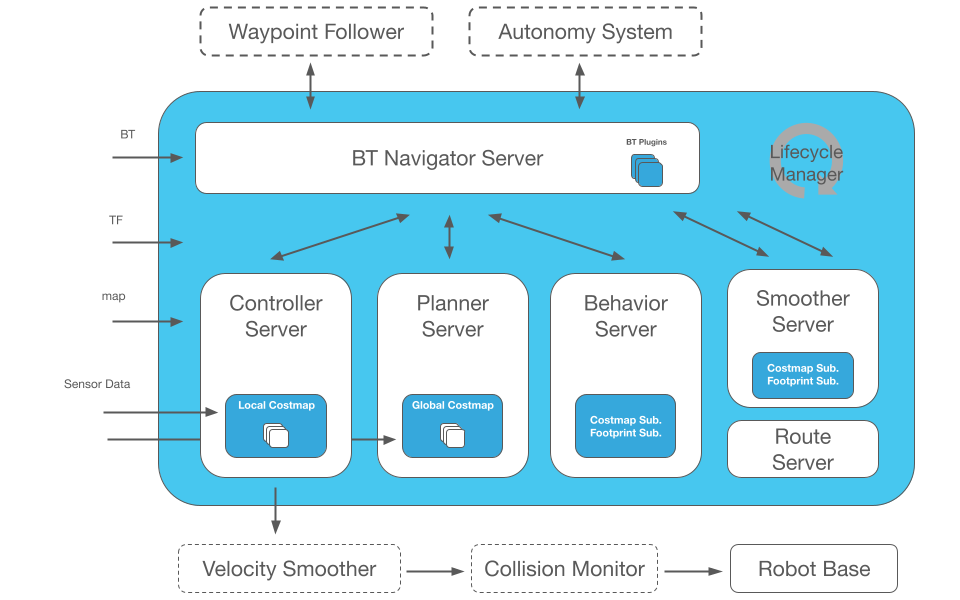
\includegraphics[width=0.8\textwidth]{nav2_architecture.png}
    \caption{NAV2 stack architecture \cite{nav2_architecture}}
    \label{fig:nav2_stack}
\end{figure}

In figure \ref{fig:nav2_stack} we can see the different components of the \gls{NAV2} stack required for 
robust autonomous behaviour. The main components are thr Controller server, which is responsible for, using a controller 
plugin, controlling the robot's movement, the Planner server, which is responsible for, using a custom plugin, 
planning the robot's path, the Behaviour server which, given a custom behaviour tree, is responsible for selecting the 
next action to be taken by the robot, the BT Navigator server, which coordinates all the other servers and the Lifecycle manager 
which controls the lifecycle of the different modules mentioned previously. The stack also includes a variety of already 
defined plugins to be used for localization, path planning and control, however, in this work, a custom planner, controller, 
behaviour tree and also state publisher are created to suit the specific needs of the robot.

\section{Environment}
\label{subsec:environment}
\paragraph{}For development purposes, a virtual environment is used to develop the navigation software 
and test it without the need for a physical robot. This environment can be created using Gazebo, a 
robotics simulator that is compatible with \gls{ROS2}, and it allows the user to create a world in xml format, specifying 
the different physical properties of the environment as well as the structures and objects inside it.

Since the robot will be operating in an agricultural environment, the world created for 
the simulation would have to reflect that, so a simple world was created with five 
corridors with traffic bariers on each side (to simulate trees or crops) and some additional 
obstacles to make for a more complex environment.
\begin{figure}[H]
    \centering
    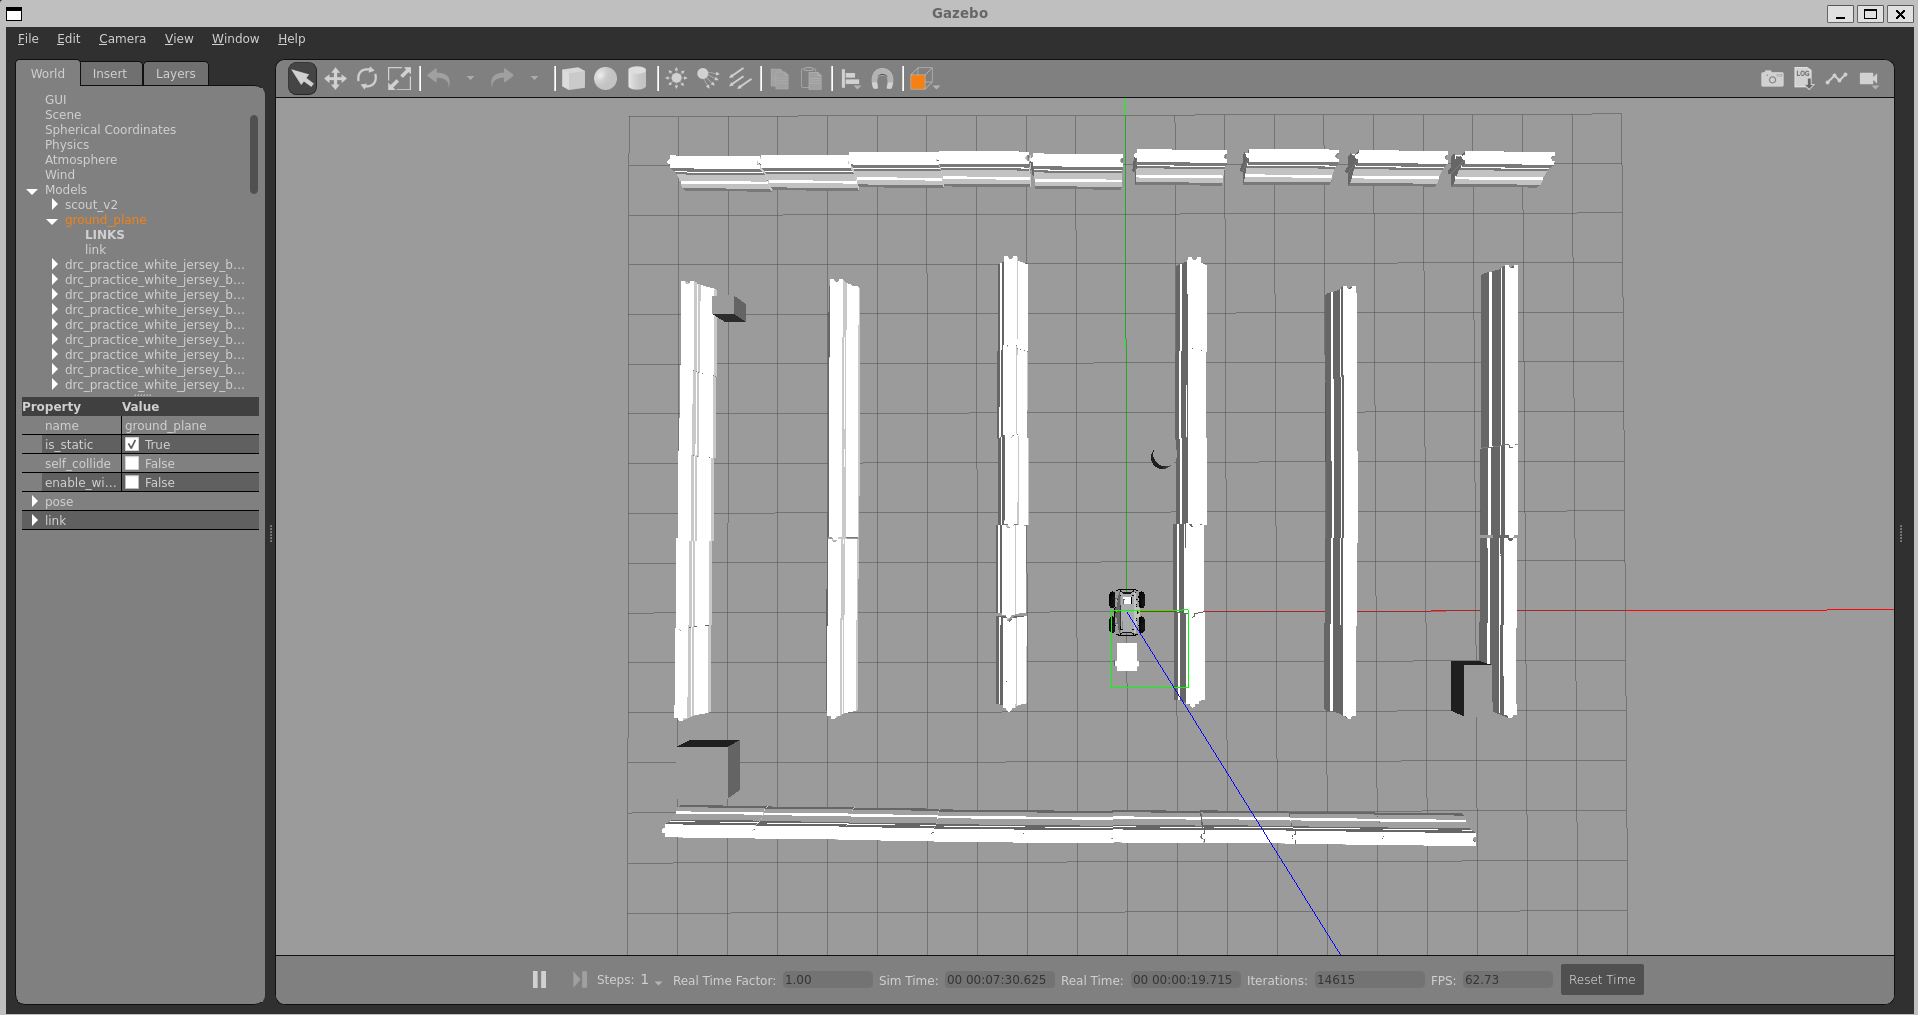
\includegraphics[width=0.9\textwidth]{gazeboworld.png}
    \caption{Gazebo world used for simulation.}
    \label{fig:gazebo_world}
\end{figure}

Having the world isn't enough to have a fully autonomous robot, a map 
of the world is also required for the localization and navigation components to work. 
this map can be created using the \gls{SLAM} algorithm, as mentioned in the previous chapter \ref{sec:slam}. 
Since the \gls{NAV2} stack already has a package that implements the \gls{SLAM} algorithm, all it needs is to 
have the robot's model and sensors running in the environment, and it will create a map.
The robot model used in this work is fortunately made available by its manufacturers 
so it can be used in the simulation directly, and the sensors are simulated using their 
Gazebo plugins, which allow the user to specify the sensor's properties, such as range, resolution, and noise.

\begin{figure}
    \centering
    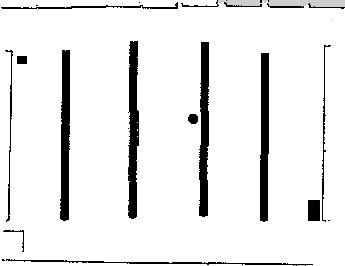
\includegraphics[width=0.9\textwidth]{wall_map.png}
    \caption{Map created using the SLAM Package in the Gazebo Simulation. White space is non-occupied space, black are obstacles and grey is undiscovered space.}
    \label{fig:slam_map}
\end{figure}

The map shown in figure \ref{fig:slam_map} is the result of mapping the simulated environment, 
however, since this work aims to have an operational prototype, two other maps were created 
in real world locations, one in a concealed room and another in a corridor with a few obstacles to simulate the rows 
of crops. 

These last two maps, due to being created in real world locations, can't be 
simulated in gazebo, so the hardware interface for the robot and its sensors 
would need to be implemented in order to comunicate within the \gls{ROS2} framework. 
Fortunately the necessary packages were all provided by the manufactures \cite{ScoutRepo, RoboSense} and only needed a few adjustments to 
be completely integrated witin the system. Since the LIDAR used is a 3D LIDAR, the output 
of the sensor is a point cloud, however, the \gls{SLAM} package used outputs 2D Maps and would need a 
Laser Scan to be used. To overcome this a \gls{ROS2} package was used (Pointcloud to Laser Scan) that 
given the distance and angles that need to be covered, converts a point cloud into a laser scan, 
allowing for the \gls{SLAM} package to work as intended.
\begin{figure}[H]
    \centering
    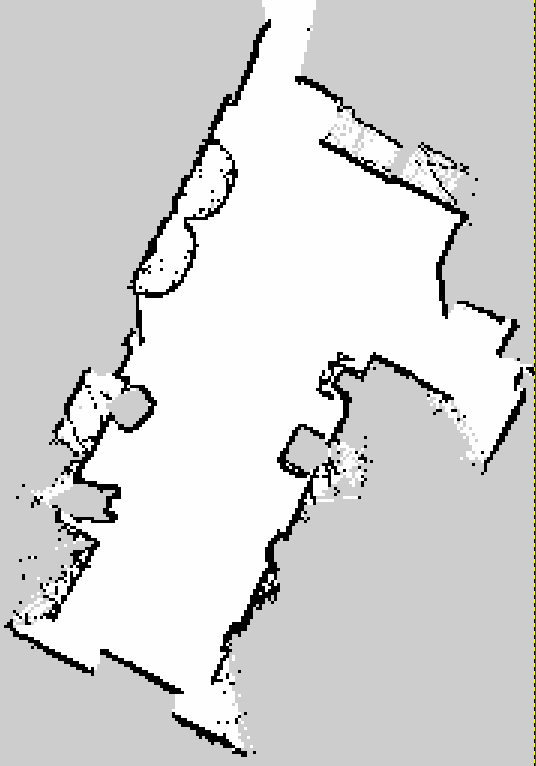
\includegraphics[width=0.50\textwidth]{basement.png}
    \caption{Map of the concealed room.}
    \label{fig:basement_map}
\end{figure}
\begin{figure}[H]
    \centering
    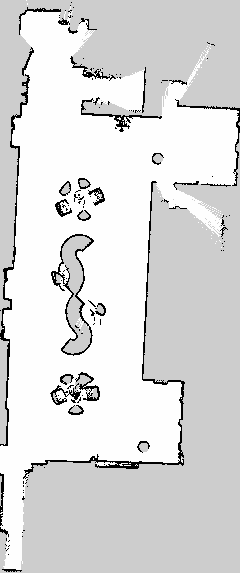
\includegraphics[width=0.65\textwidth]{corridor_map.png}
    \caption{Map of the corridor.}
    \label{fig:corridor_map}
\end{figure}

To visualize the robot in these maps as well as all the different data that is deemed relevant, a software called 
Rviz2 is used. This software allows the user to select the various \gls{ROS2} topics that are being published 
by the running nodes and visualize them in a 3D environment, which is very useful for debugging and testing purposes.
\begin{figure}[H]
    \centering
    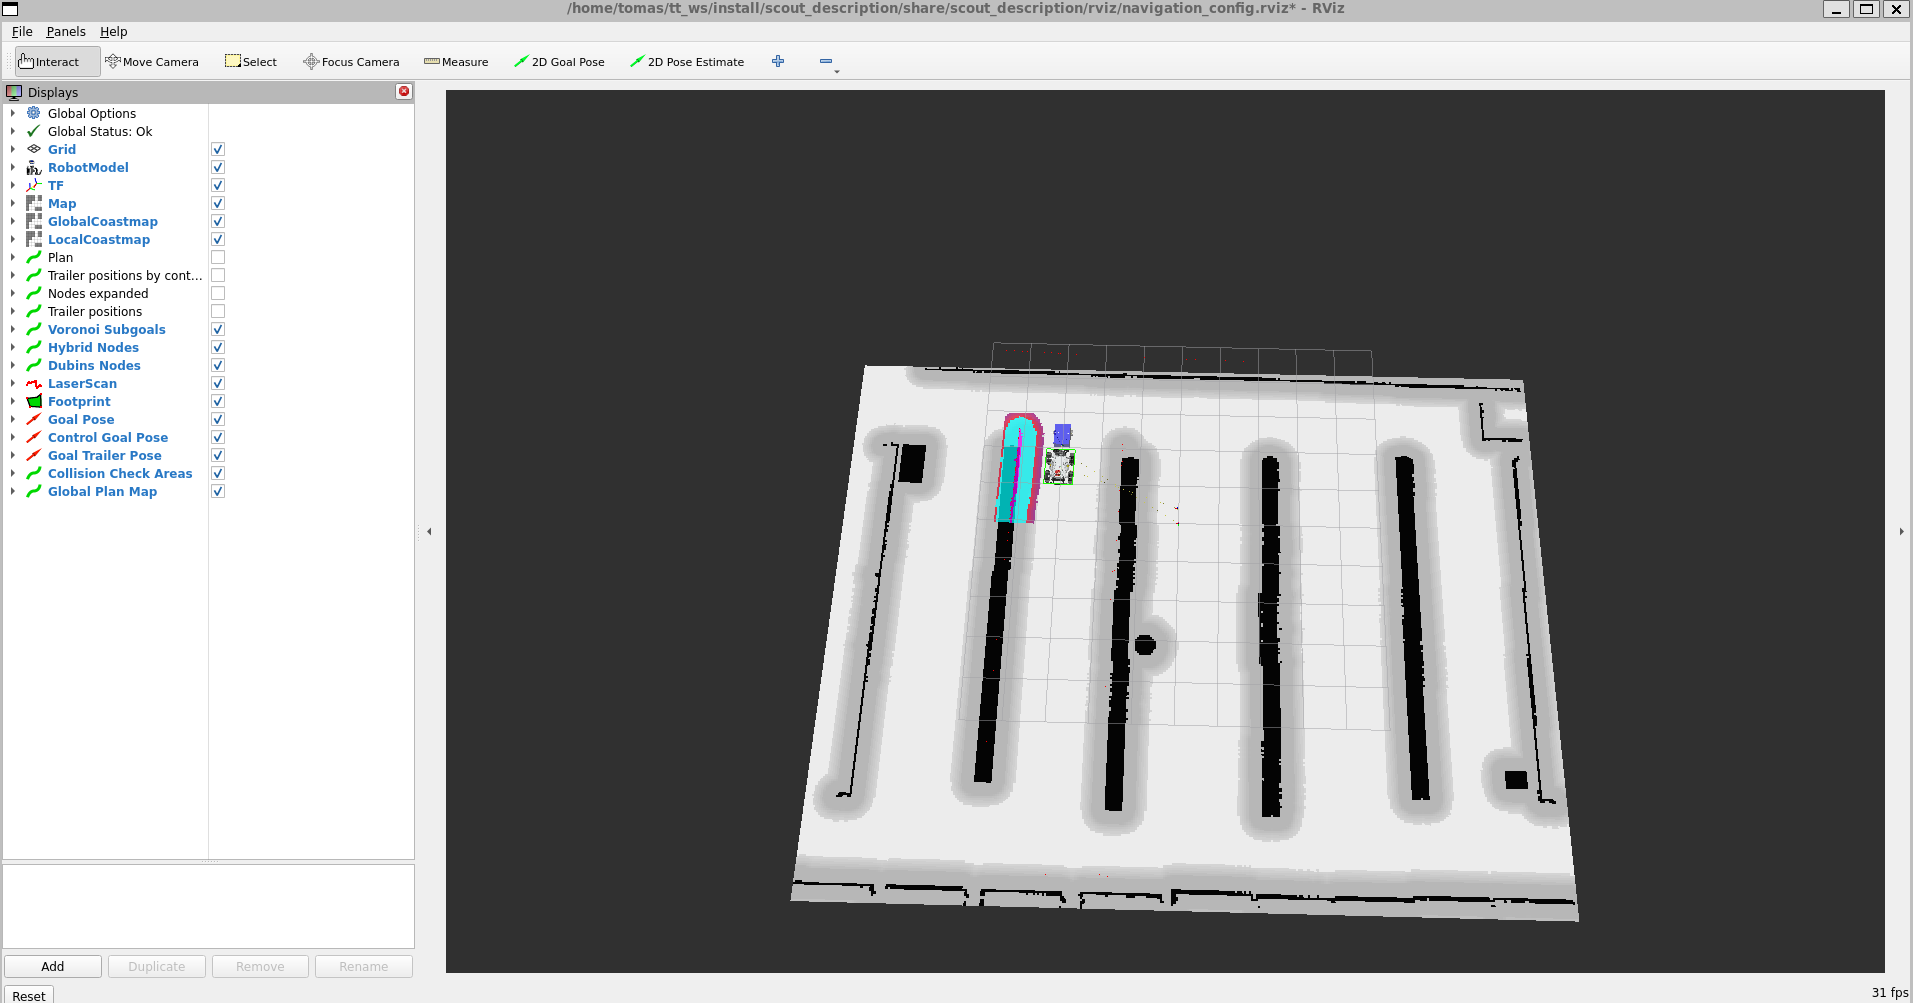
\includegraphics[width=0.9\textwidth]{Rviz2viz.png}
    \caption{Rviz2 visualization of the robot in the simulated environment.}
    \label{fig:rviz2_visualization}
\end{figure}

The figure \ref{fig:rviz2_visualization} shows, at the left, the different data provided by the developed system and, above it the 
navigation tools like estimatin the robot's initial position and goal generation. These last two tools can be used manually 
in Rviz2 or be published by a custom node if the user requires it.

\section{Planning algorithm}
\label{sec:planning_algorithm}

\paragraph{}As explained in the previous chapter \ref{sec:planner1}, 
the planner is devided into three main components, the Voronoi Graph, the Dubins Path and the Hybrid A* recovery algorithm.

\subsection{Voronoi Graph}
\label{subsec:voronoi_graph}

\paragraph{}The main function of the Voronoi Graph is to create a set of points in space that can be searched for a  
simple path to the goal using an A* search. Due to the nature of calculating a Voronoi Graph, it can be very computationally 
expensive, so the algorithm is ran offline, when the environment is mapped, and the resulting graph is saved to a 
file for the online planner to use. To create this graph, a Ros2 python node was created that executes a script with 
the previous behaviour.

The algorithm first works by creating black and white image containing the edges of the obstacles and grouping them 
into a single column of points which are then used to calculate the Voronoi Graph using the 
Scipy library \cite{Scipy}. 
This graph is then filtered to remove points that are inside the obstacles and remove points that are too close to each other. Points can be created inside the obstacles 
because of their width, so the algorithm considers it available space. To filter them, they are 
place on the original map, and  if they're not in white space, they're removed.
\begin{figure}[h]
    \centering
    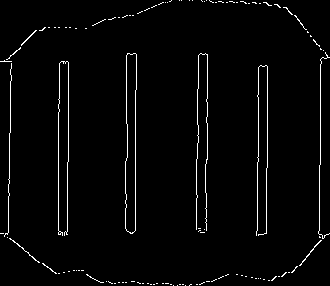
\includegraphics[width=0.7\textwidth]{edges_map_V20.png}
    \caption{Image with the obstacle edges.}
    \label{fig:voronoi_edges}
\end{figure}
\begin{figure}[h]
    \centering
    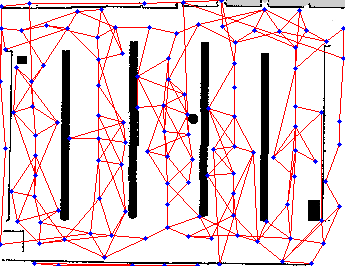
\includegraphics[width=0.7\textwidth]{voronoi_graph_V100.png}
    \caption{First Voronoi Graph created for the environment in figure \ref{fig:gazebo_world}.}
    \label{fig:voronoi_graph1}
\end{figure}

It is possible to verify that the graph isn't exacly perfect, as it doesn't 
show the usual behaviour of a Voronoi Graph with straight lines equidistant to the 
obstacles, however, this is due to the jagged nature of the edges of the obstacles, creating 
several equidistant points. Dispite thos, this graph is pourly dense in some 
areas compared to others, so a second iteration is made to correct this.
\begin{figure}[h]
    \centering
    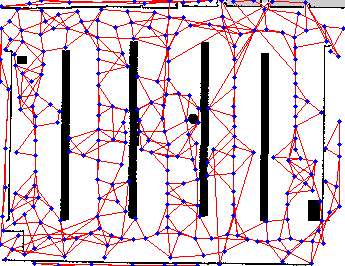
\includegraphics[width=0.8\textwidth]{voronoi_graph_V101.png}
    \caption{Second Voronoi Graph created for the environment in figure \ref{fig:gazebo_world}.}
    \label{fig:voronoi_graph2}
\end{figure}

An then finalized with a third iteration that now resembles a more 
traditional Voronoi Graph.
\begin{figure}[h]
    \centering
    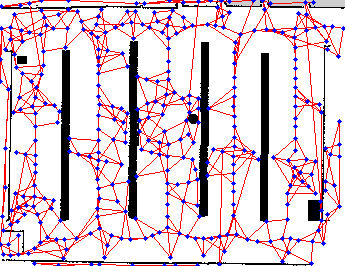
\includegraphics[width=0.8\textwidth]{voronoi_graph_V102.png}
    \caption{Final Voronoi Graph created for the environment in figure \ref{fig:gazebo_world}.}
    \label{fig:voronoi_graph3}
\end{figure}

It is now possible to verify the straight segments between the obstacles in the 
less obstacle dense areas, which allows for more efficient path planning. The denser areas 
having more nodes and edges allows for more pathing options which is useful 
for obstacle avoidance. The nodes and edges are then saved to a file to be 
then used by the planner.
\begin{figure}[h]
    \centering
    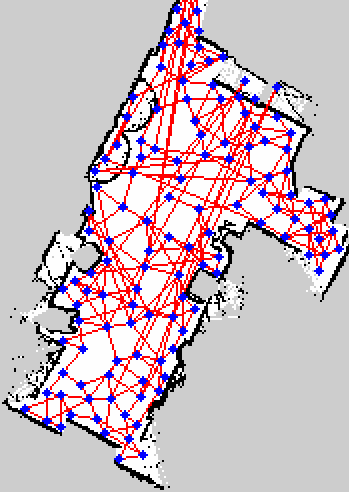
\includegraphics[width=0.9\textwidth]{basement_graph_002.png}
    \caption{Concealed room Graph.}
    \label{fig:basement_graph_002}
\end{figure}
\begin{figure}[h]
    \centering
    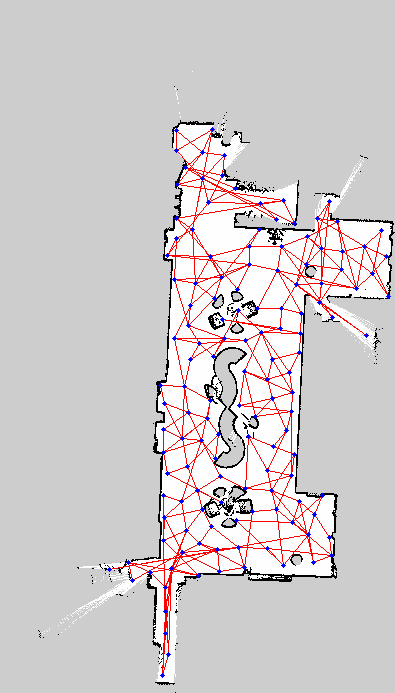
\includegraphics[width=0.85\textwidth]{corridor_graph_009.png}
    \caption{Corridor Graph.}
    \label{fig:corridor_graph_009}
\end{figure}
\clearpage

Once again, the Vorronoi Graphs aren't the usual straight line ones however, the environments 
used are not simple and have several obstacles leading to irregular graphs.

\subsection{Planner Plugin}
\label{subsec:planner_plugin}
\paragraph{}As mentioned in the subsection \ref{subsec:navigation2}, the \gls{NAV2} stack allows for the creation of custom plugins that are 
used by the different servers to perform their tasks. In this case, a custom planner plugin was 
created to be used in the Planner server, responsible for creating a global plan 
for the robot to follow. This plugin is written in C++ and uses the 
\gls{NAV2} plugin interface to be recognized by the BT Navigator server.

The plugin is responsible for the Dubins Path and Hybrid A* recovery algorithm, 
as well as the A* search algorithm that is used to find the path between the start and goal points. It is done 
by reading the file with the Voronoi Graph, verifying the closest nodes to the 
start and goal points, and then searching for the path. The resulting subpath is 
shown in figure \ref{fig:subgoals} visualized in Rviz2.
The reason this path cannot be used directly is because it is not a continuous 
smooth path, it is a set of points that serve as heuristic for the planner and 
some points could be connected in ways that are not feasible for the robot, such as reversing, and, therefore, 
a Dubins Path needs to be created.
\begin{figure}[h]
    \centering
    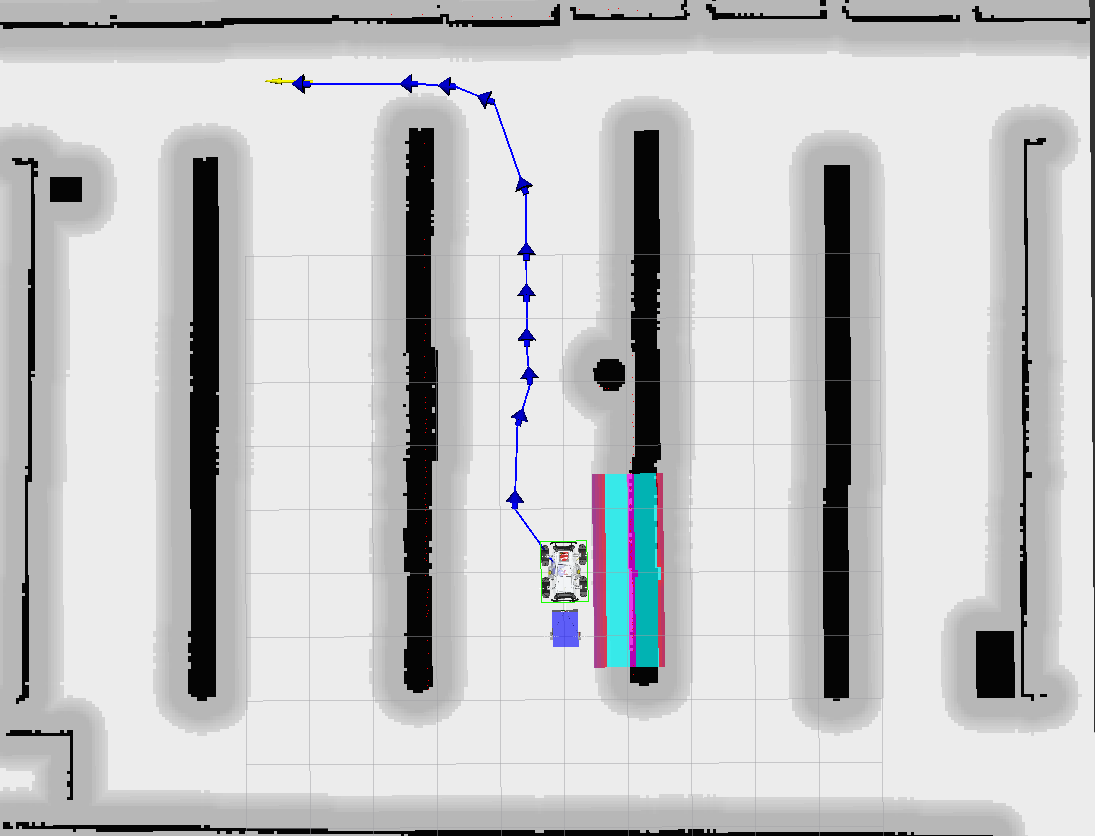
\includegraphics[width=0.9\textwidth]{subgoals.png}
    \caption{Subpath, in blue, created by the planner plugin.}
    \label{fig:subgoals}
\end{figure}

The Dubins Path, explained in \ref{sec:dubins_path}, is then created using the start and goal points, as well as the desired 
turning radius for the robot, this could be set from a configuration file and 
given to the plugin when created.

A feature of the planner is the addition of the trailer. The planner needs to take into account 
the position of the trailer to ensure that no collisions occur while the robot is 
following the path. However, the \gls{NAV2} stack has a limitation. There's a package 
within the stack that allows for the calculation of the robot's joint values, the joint state 
publisher. This package takes in the robot's model, described in a \gls{URDF} file, and calculates the joint values 
based on the robot's movement. However this package does account for passive revolute joints, like 
the trailer connector or trailer hitch. Not accounting for this would mean 
that the trailer would either not be considered, which wouldn't make sense 
as it is the whole purpose of this robot, that the trailer would be considered 
fixed to a certain position, however this solution would not be feasible as it might make 
some curves impossible to follow, so a custom publisher was made to publish the trailer's hitch 
transform based on the trailer's movement. 